%%
%  ******************************************************************************
%  * #file    Szablon_raportu_EN_Latex.tex
%  * #author  Adrian Wójcik   adrian.wojcik(at)put.poznan.pl
%  *          
%  * #commit  Patryk Kościk   koscikpatryk(at)gmail.com
%  *          Modified the template for Projekt przejsciowy purposes          
%  *          
%  *
%  * #commit  Patryk Kościk   koscikpatryk(at)gmail.com
%  *          Zupełnie przewrócono na łeb formatke po taktycznym wyjasnieniu          
%  *          
%  * #version 1.1
%  * #date    09-Mar-2022
%  * #brief   PROJPRZEJ
%  *
%  ******************************************************************************
%%  
\documentclass[11pt, a4paper]{article}

\usepackage{SM_template}

% Wypełnijcie te dyrektywy zgodnie z waszym tematem
%
% \lab      -> NAZWA CZUJNIKA,          np.: 'DHT22'
% \comment  -> Króciutki opis co to,    np.: 'Cyfrowy czujnik temperatury'
% \author   -> Autor dokumentu          np.: Patryk Kościk
%
% Pamiętajcie o zmianie ścieżki w \addbibresourcue (!)

\lab{Moduł KY-020}
\comment{Cyfrowy czujnik przechylenia. }
\author{Anna Nasierowska}
\addbibresource{bib/Czujnik_przechyleniaKY020.bib}

%
% Początek dokumentu
%
\begin{document}

%
% Strona tytułowa
%
\mainpage{{Czujnik_przechylenia_KY020/czujnik_tytul}}
\newpage

\section*{Opis elementu} \addcontentsline{toc}{section}{Wstęp}
Omawiany detektor przechylenia to prosty cyfrowy czujnik, składający się z 3 pinów, wbudowanego rezystora oraz części wystającej, która odpowiada za wykrycie odchylenia. Jest to mały moduł, który można napotkać np. w zestawach czujników do arduino. 


\vspace{0.5cm}
\begin{figure}[h]
\centering
\begin{subfigure}{.5\textwidth}
  \centering
  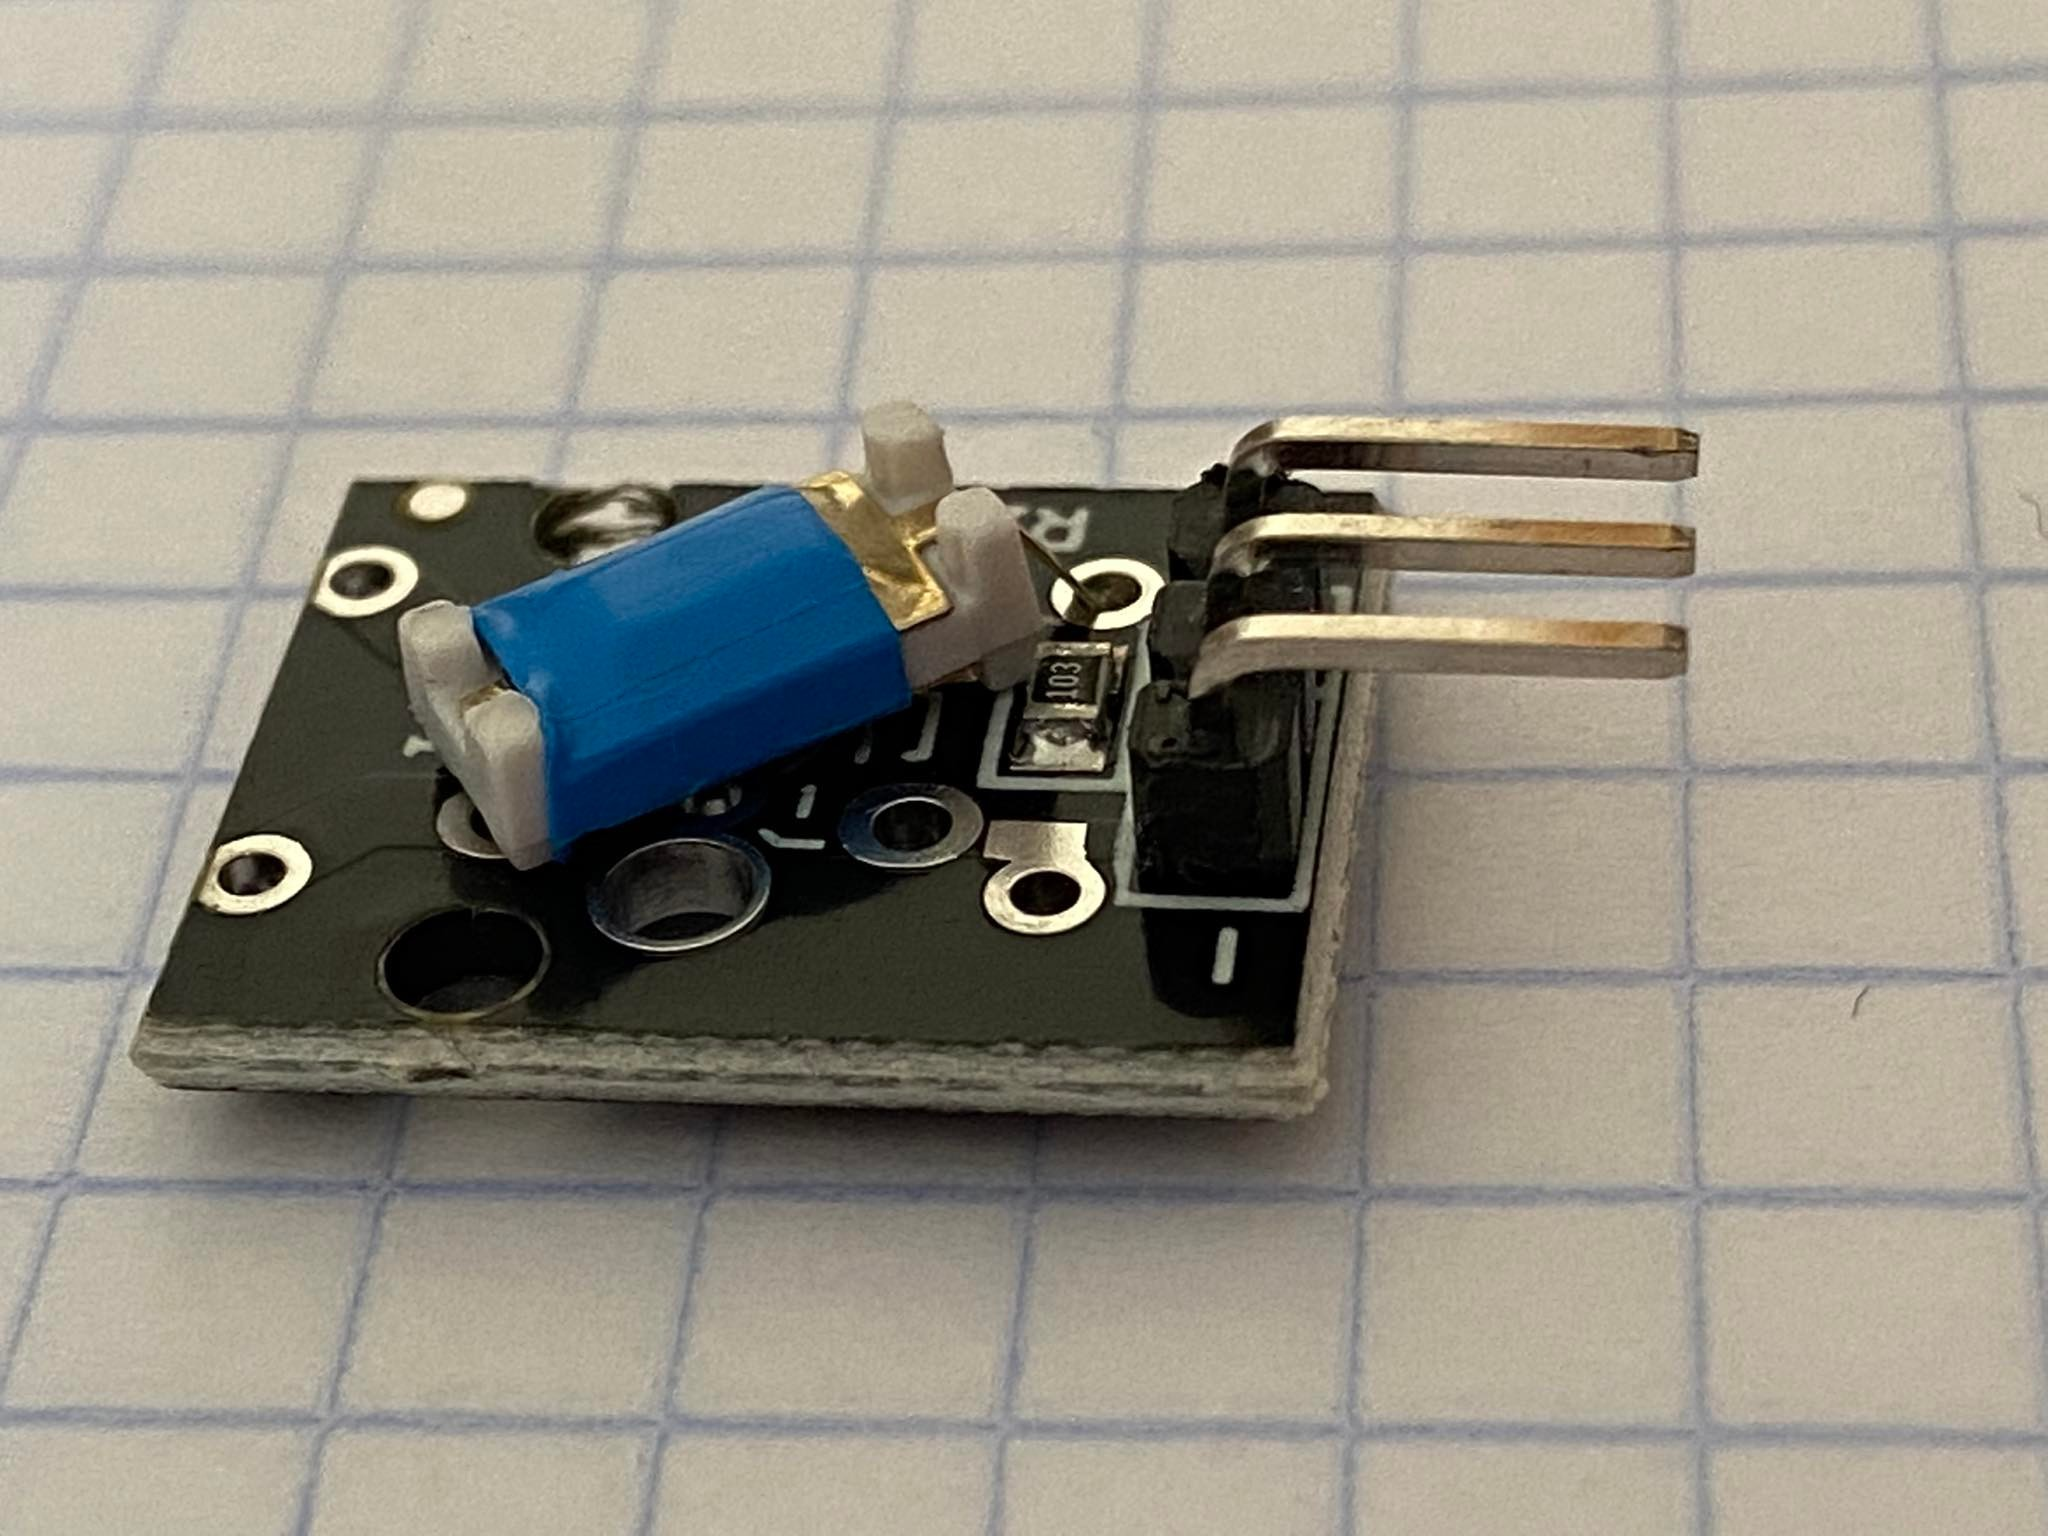
\includegraphics[width=.5\linewidth]{fig/Czujnik_przechylenia_KY020/zdj_modułu/czujnik_img1.jpg}
  \caption{Zdjęcie czujnika}
  \label{fig:sub1}
\end{subfigure}%
\begin{subfigure}{.5\textwidth}
  \centering
    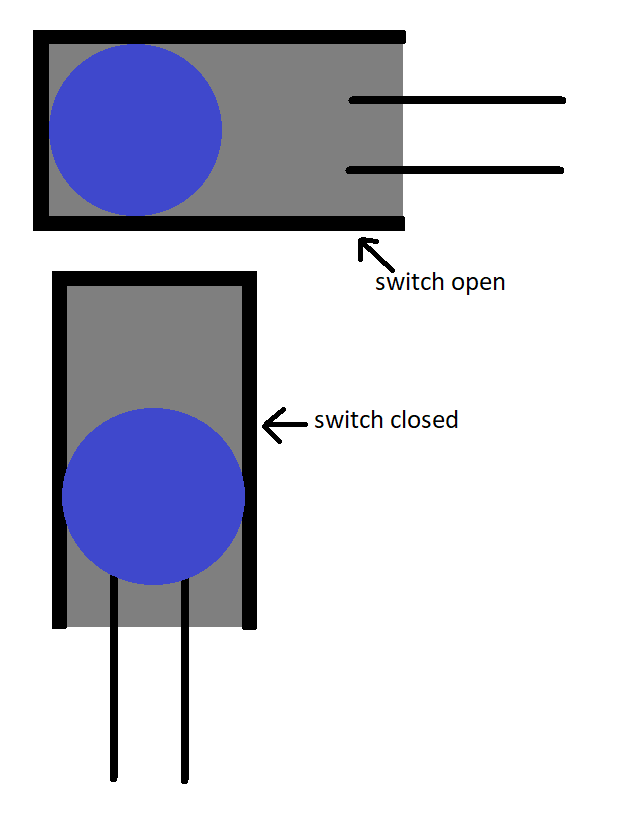
\includegraphics[width=.4\textwidth]{fig/Czujnik_przechylenia_KY020/zasada_dzialania/schemat.png}
      \caption{Zasada działania}
  \label{zd}
\end{subfigure}
\caption{}
\label{fig:test}
\end{figure}
\vspace{0.5cm}

Czujnik zbudowany jest w sposób widoczny na rys. \ref{zd}. W niebieskiej obudowie znajduje się metalowa przewodząca kulka, która przy nachyleniu czujnika pod odpowiednim kątem dotyka pinu 1 i 3, zamykając w ten sposób obwód. 

\vspace{0.5cm}
\begin{figure}[h]
\begin{subfigure}{.5\textwidth}
\centering
   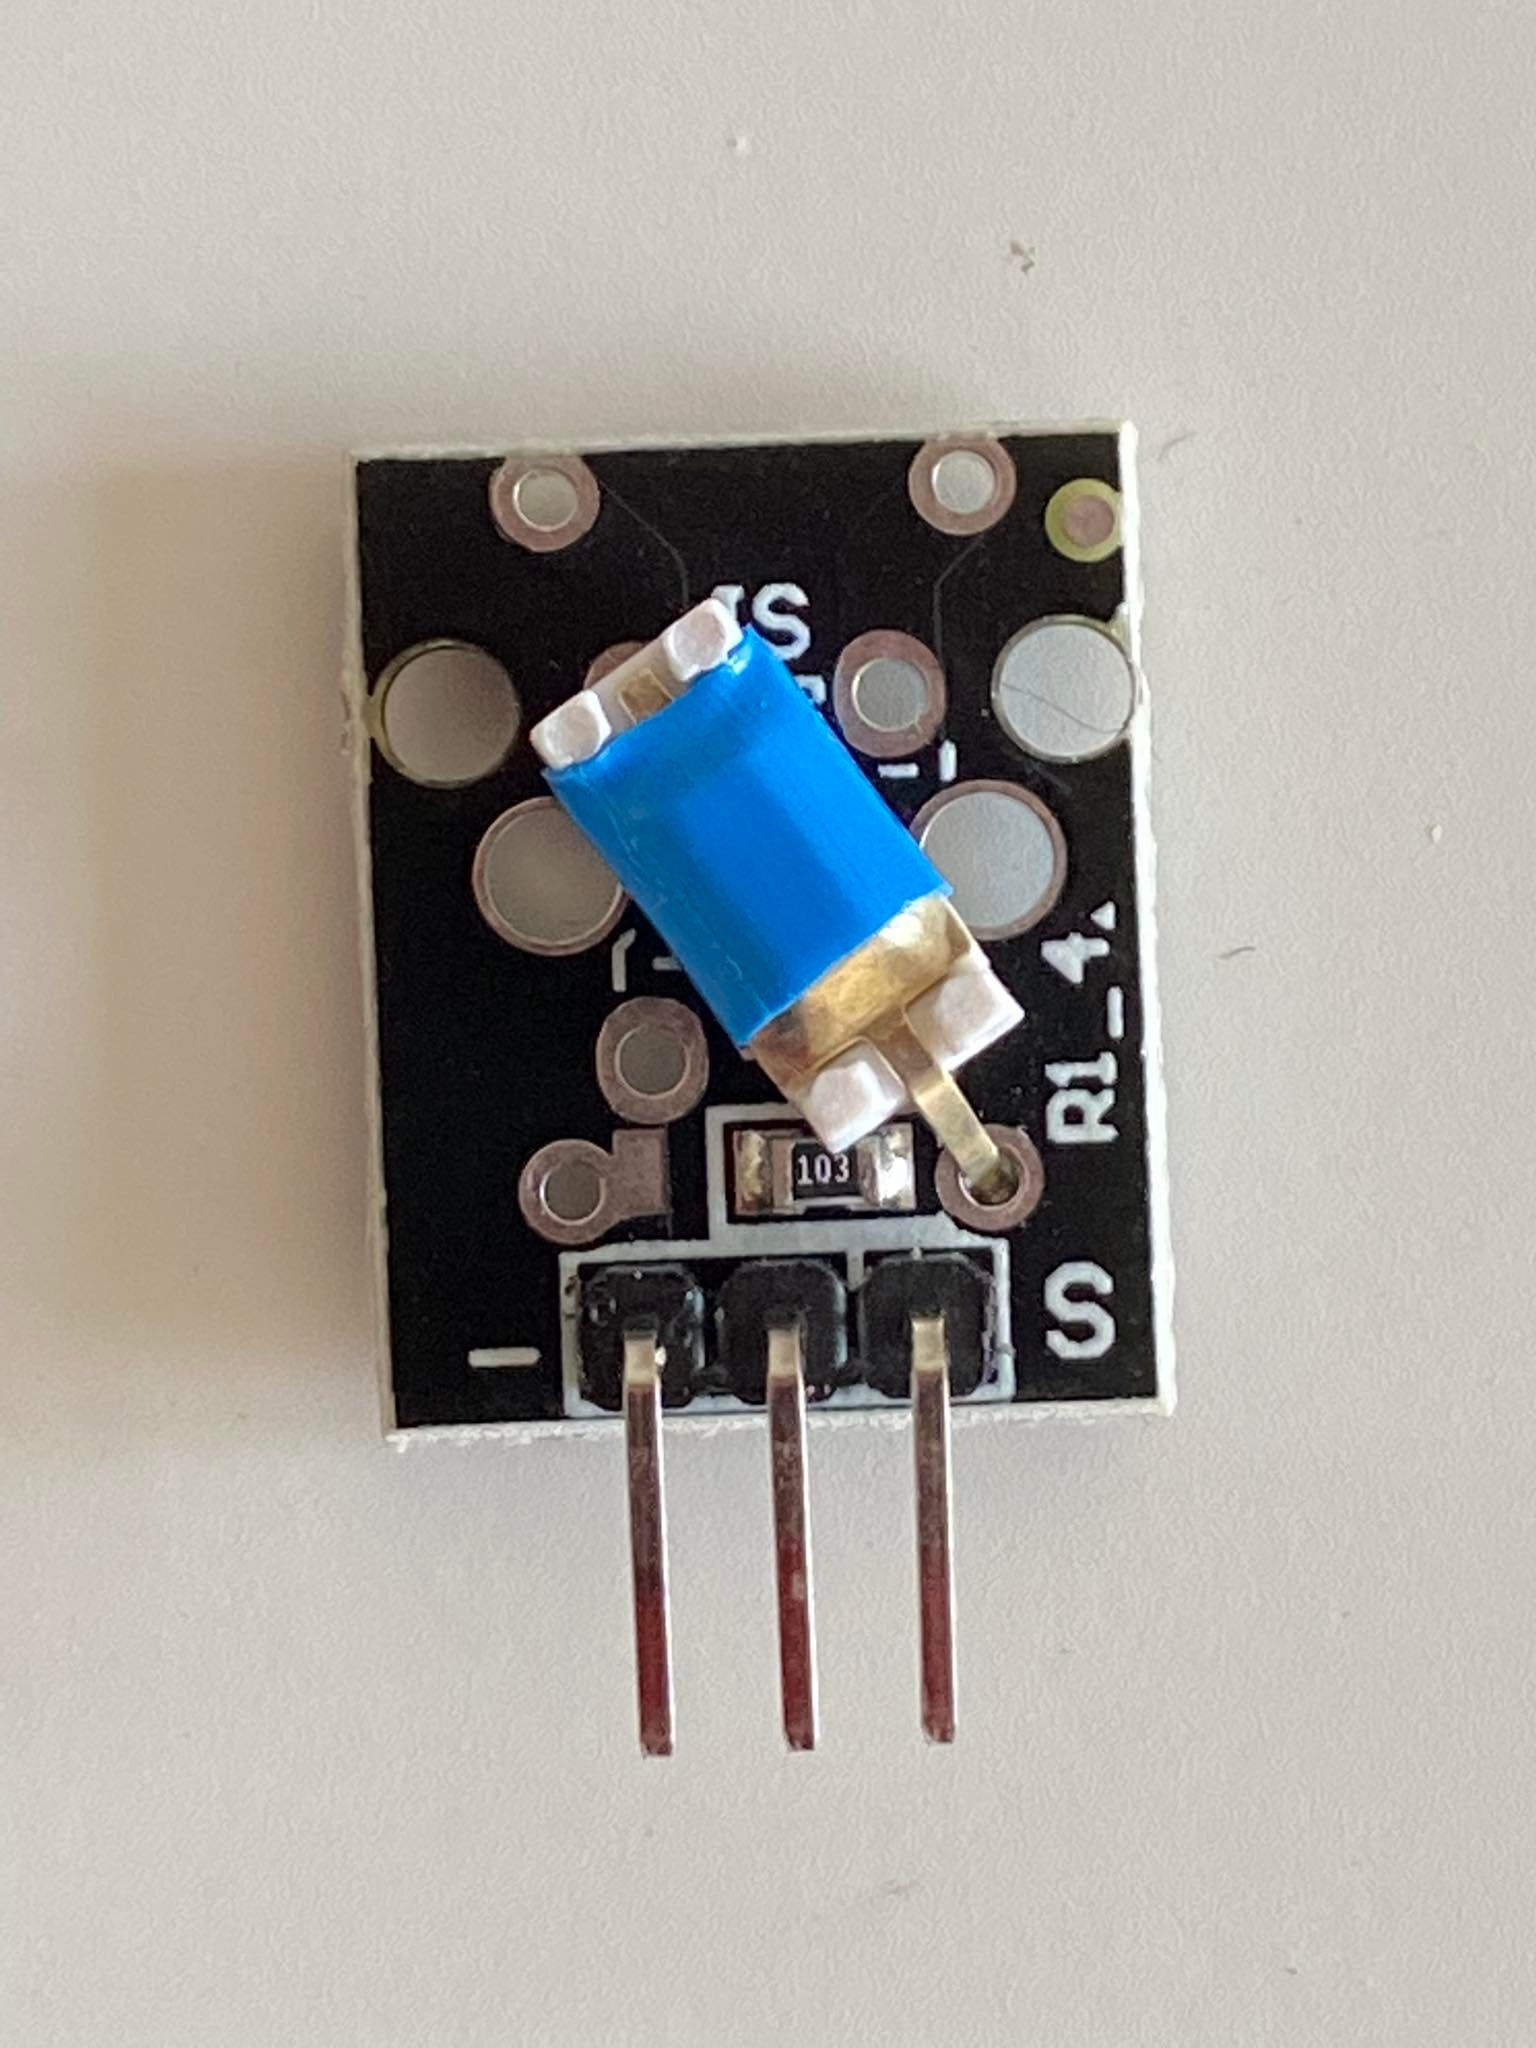
\includegraphics[width=.4\linewidth]{fig/Czujnik_przechylenia_KY020/zdj_modułu/czujnik_img2.jpg}
   \caption{Zdjęcie od góry}
  \label{fig:sub1}
  \end{subfigure}%
\begin{subfigure}{.5\textwidth}
  \centering
  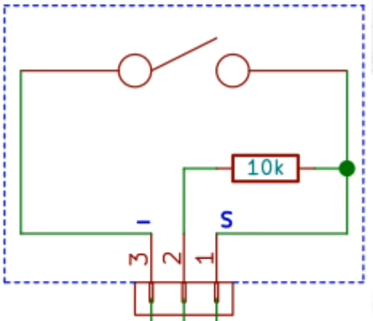
\includegraphics[width=.5\textwidth]{fig/Czujnik_przechylenia_KY020/zasada_dzialania/budowa1.png}
    \caption{Schemat}
    \label{sch}
  \end{subfigure}
  \caption{}%
\end{figure}

Powyżej opisany sposób działania sprowadza się do logiki działania przełącznika (z ang. switch), widocznego na rys. \ref{sch}.
Detektor ma 3 piny, 2 służą do podłączenia zasilania (5V) i masy(GND). Trzeci jest wyjściem czujnika, na którym pojawia się zmiana sygnału w momencie przechylenia. Dodatkowo w płytkę wbudowany jest rezystor $10k\Omega$. Kulka styka ze sobą piny 1 i 3, czyli wyjście czujnika (oznaczone literą S) z -. 
\newpage
Zastosowanie takich czujników występuje tam, gdzie ma znaczenie zachowanie go w poziomie. Jest to prosty detektor, który nie dostarcza informacji na temat kąta nachylenia. Co więcej przy bardzo małych kątach i delikatnych ruchach kulka może nie poruszyć się wystarczająco, aby zewrzeć piny. Zatem nie jest też bardzo dokładny. Czujnik może być elementem 

\begin{itemize}
    \item system wzbudzenia - można wykorzystać czujnik, aby urządzenie wychodziło z trybu uśpienia bądź oszczędzania energii w reakcji na podniesienie go z pozycji poziomej
    \item zabezpieczenia  - wstrząs lub odchylenie układu może wywoływać alarm bądź jego wyłączenie
    \item informacyjne - np. wykrycie przechylenia obiektu powoduje zapalenie się diody
\end{itemize}
\vspace{0.5cm}


\section{Użycie czujnika}
W celu zaprezentowania jego podstawowej funkcjonalności, przed podłączeniem do mikrokontrolera oraz implementacją kodu sprawdzona została ciągłość obwodu za pomocą miernika. 

\begin{figure}[h]
\centering
\begin{subfigure}{.4\textwidth}
  \centering
  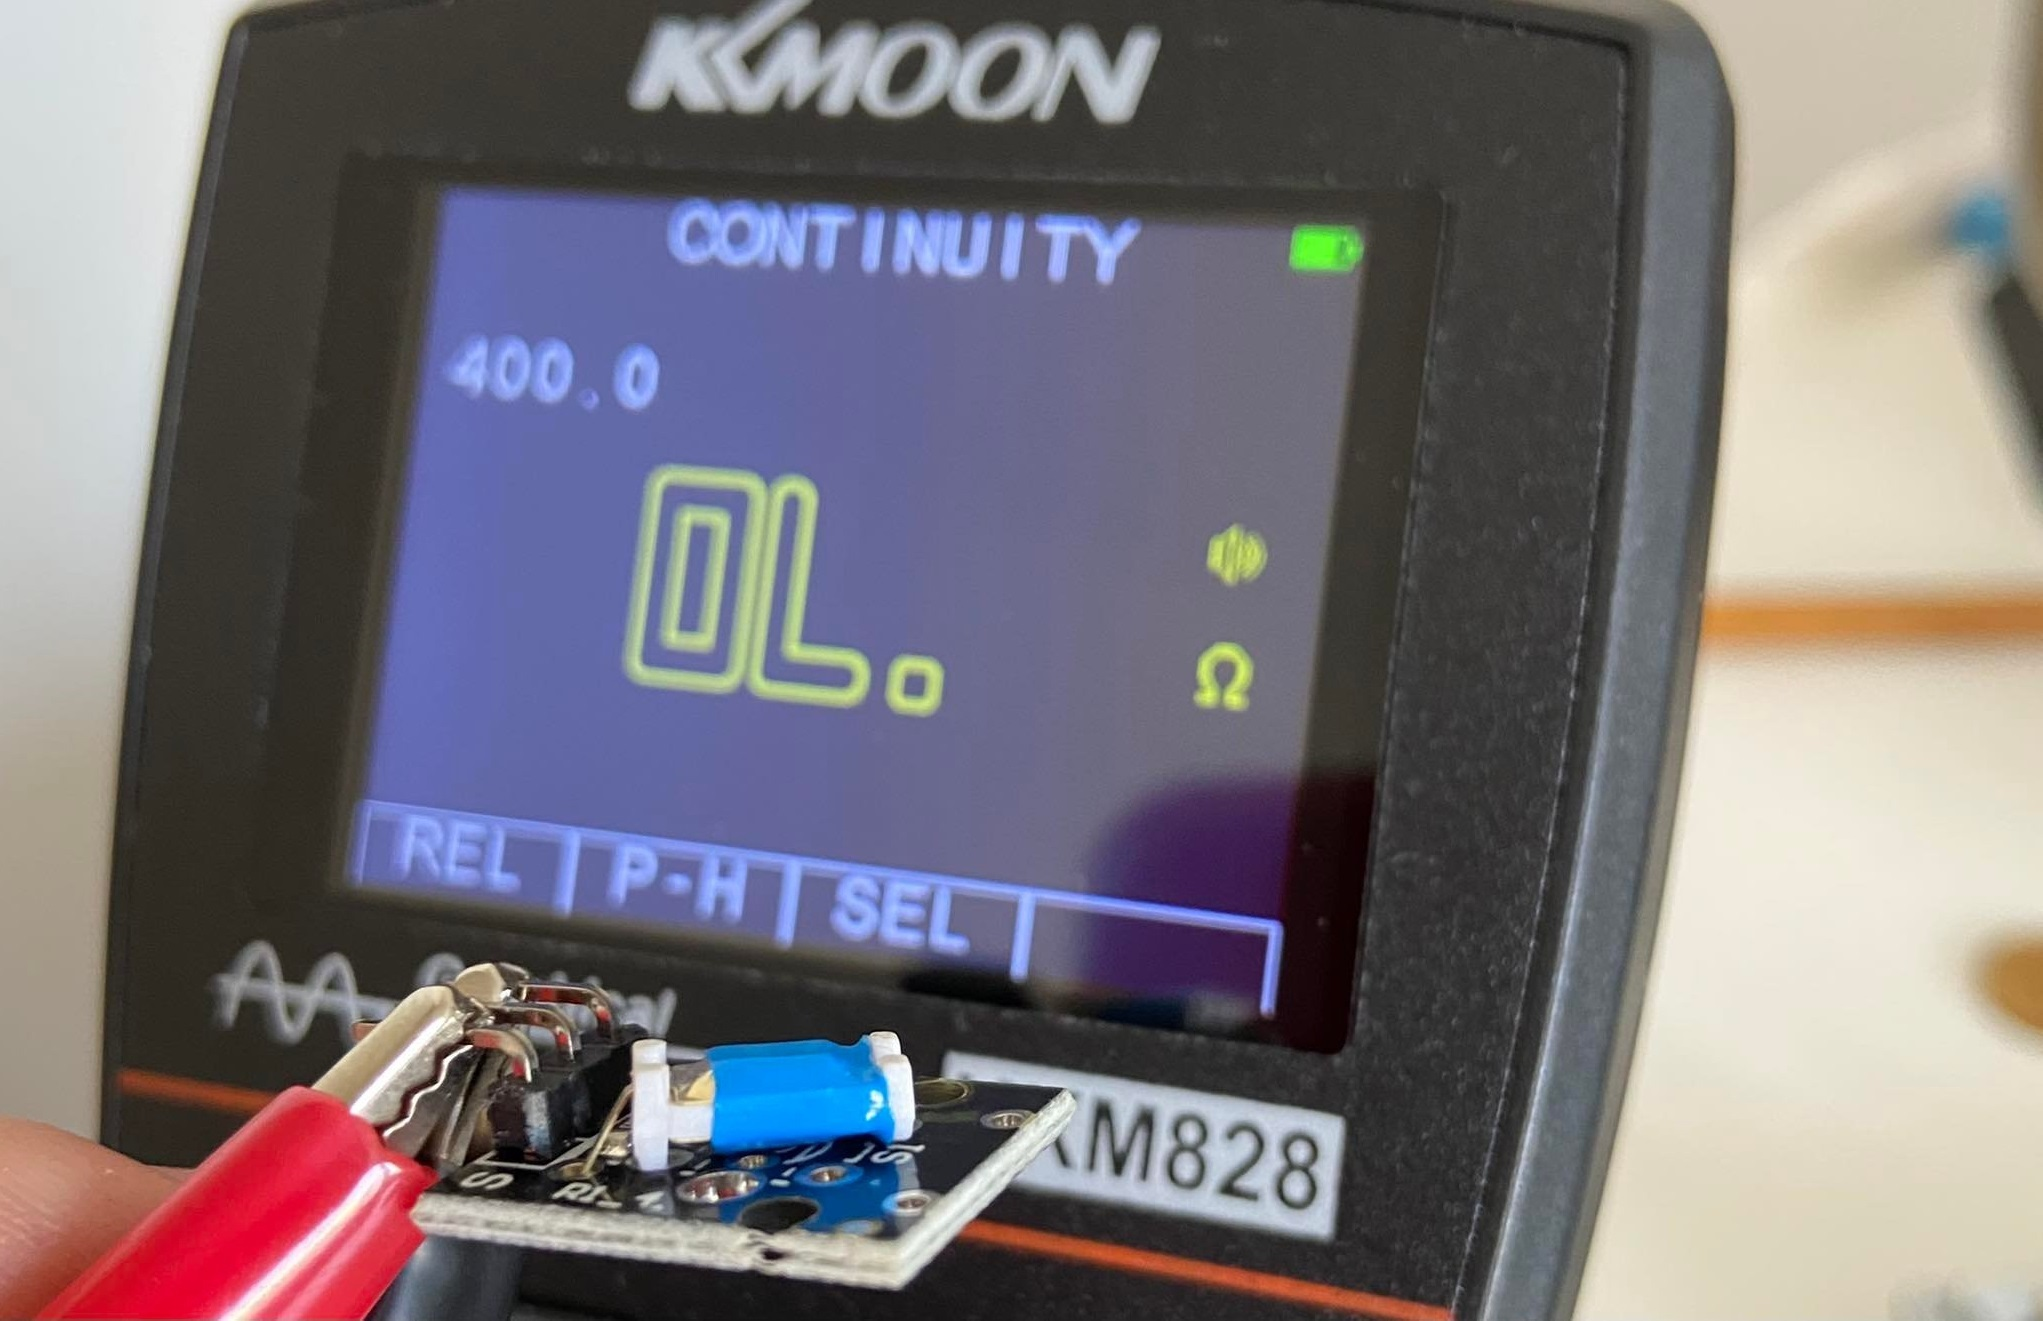
\includegraphics[width=\linewidth]{fig/Czujnik_przechylenia_KY020/działanie_ukladu/miernik1.jpg}
  \caption{Układ otwarty, moduł ustawiony poziomo.}
  \label{fig:12pd}
\end{subfigure}
\begin{subfigure}{.4\textwidth}
  \centering
  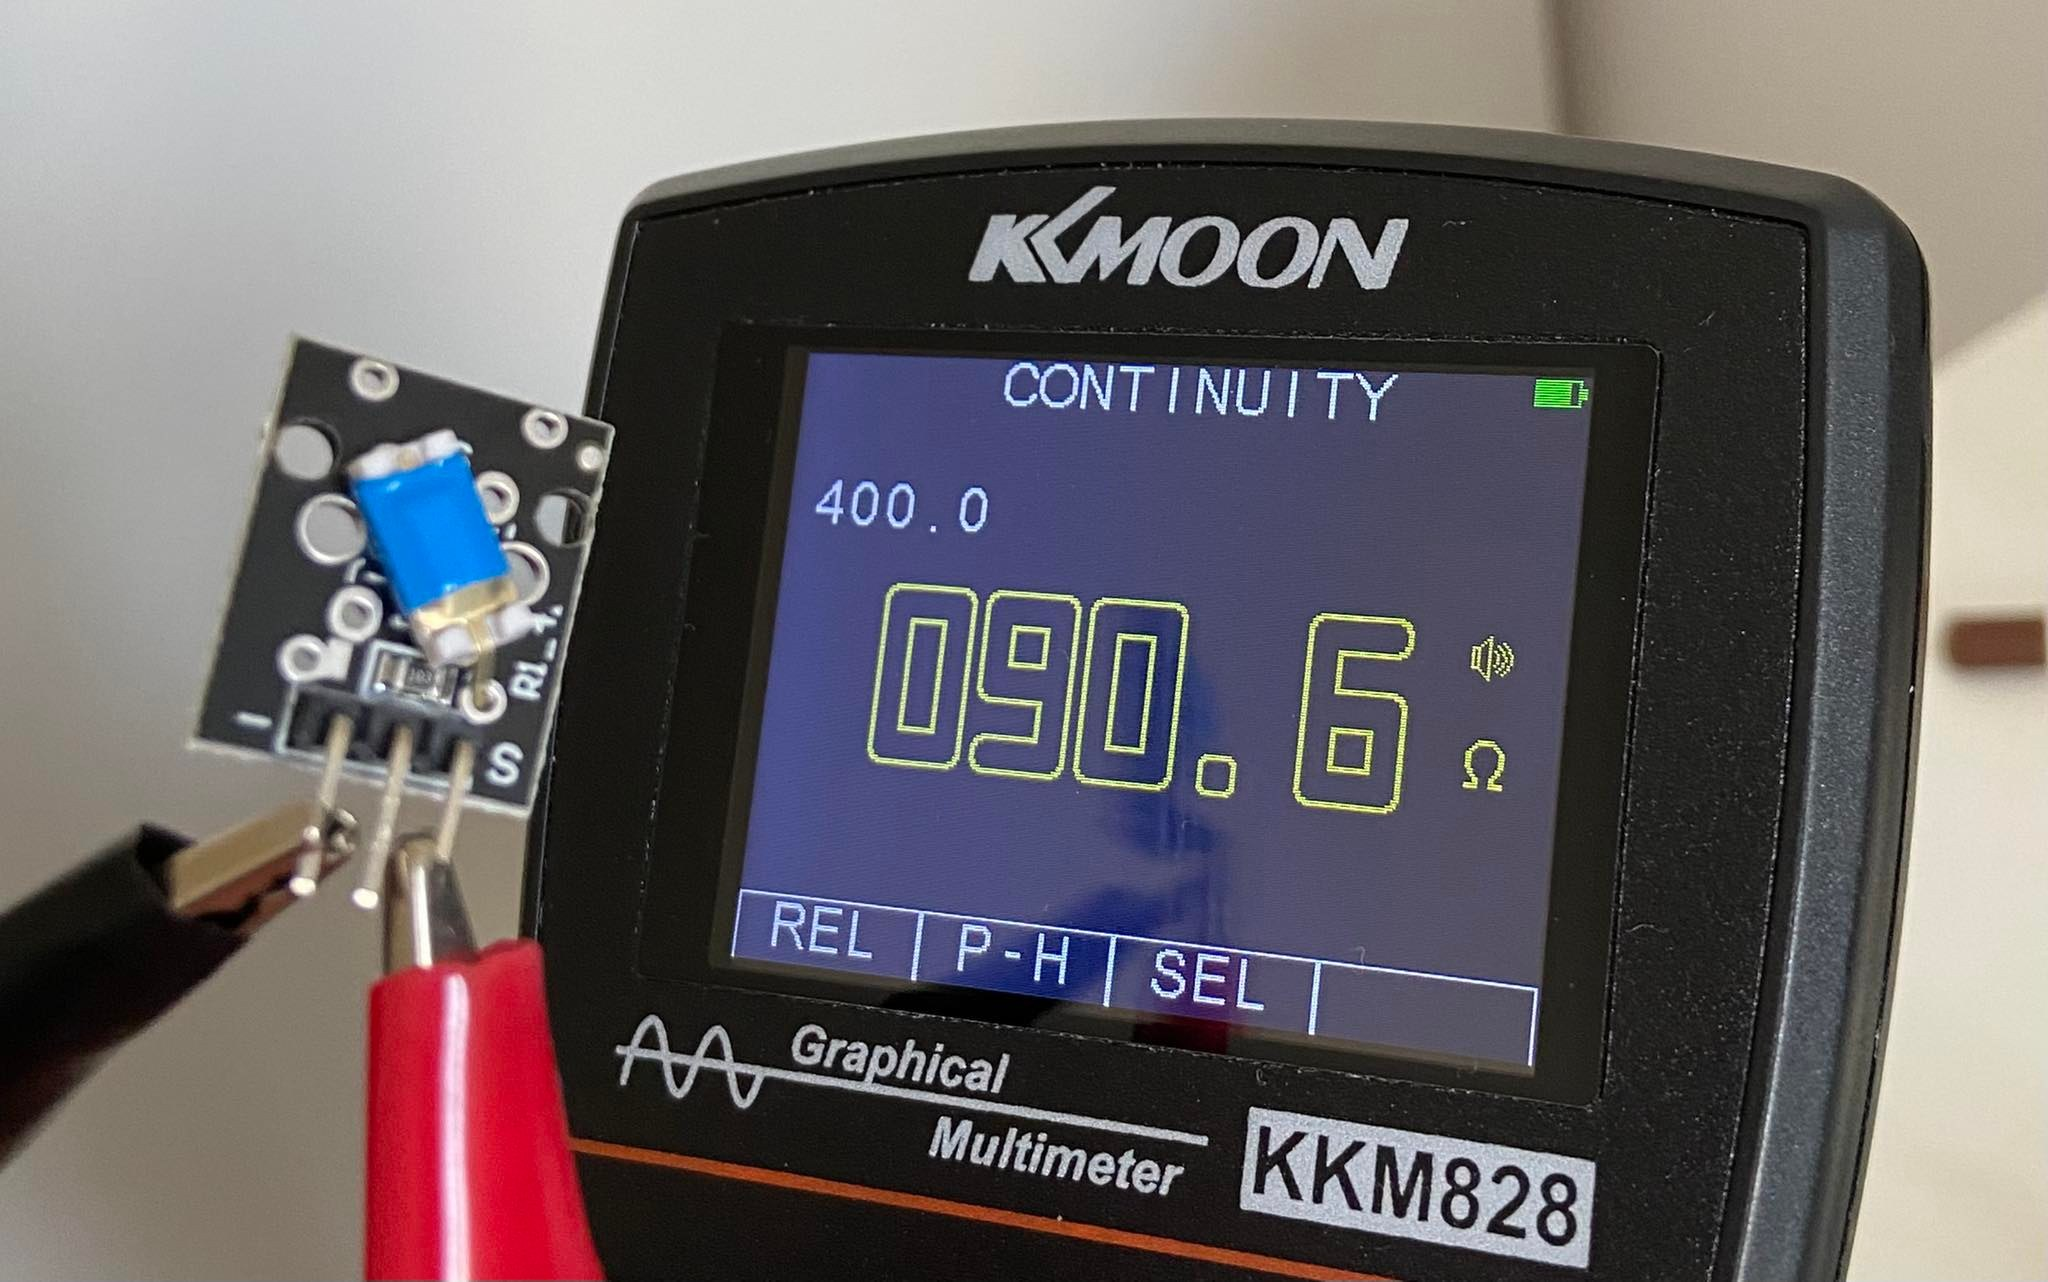
\includegraphics[width=\linewidth]{fig/Czujnik_przechylenia_KY020/działanie_ukladu/miernik2.jpg}
  \caption{Układ zamknięty, ustawienie pionowe.}
  \label{fig:sub2}
\end{subfigure}
\label{fig:12pu}
\end{figure}


Czujnik można podłączyć do mikrokontrolera na 2 sposoby, tzn. tak aby wbudowany rezystor był podciągający (pull up) lub ściągający (pull down). Zależnie od płytki u podstawy czujnika piny mogą być oznaczone w innej kolejności: przy lewym skrajnym pinie oznaczenie -, a przy prawym S lub odwrotnie.
Podczas podłączania należy zwrócić na to uwagę. \\



\begin{figure}[h]
\centering
\begin{subfigure}{.4\textwidth}
  \centering
  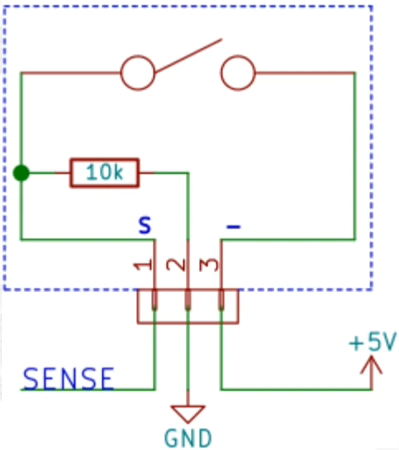
\includegraphics[width=.5\linewidth]{fig/Czujnik_przechylenia_KY020/polaczenie_modulu/12_pulldown.png}
  \caption{Rezystor ściągający.}
  \label{fig:12pd}
\end{subfigure}
\begin{subfigure}{.4\textwidth}
  \centering
  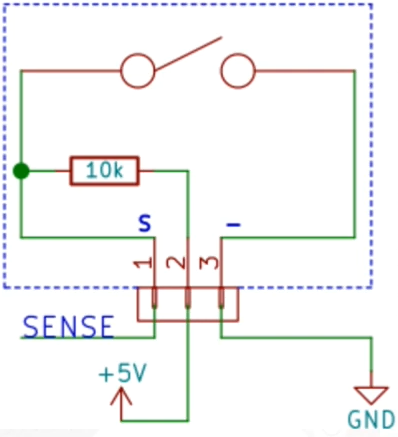
\includegraphics[width=.5\linewidth]{fig/Czujnik_przechylenia_KY020/polaczenie_modulu/12_pullup.png}
  \caption{Rezystor podciągający.}
  \label{fig:sub2}
\end{subfigure}
\caption{Połączenie elektryczne.}
\label{fig:12}
\end{figure}

%
%\vspace{0.5cm}
%\begin{table}[h!]
%    \centering
%    \begin{tabular}{|c|c|c|c|} 
%        \hline
%        \multicolumn{2}{|c|}{NUCELO-F767ZI} & \multicolumn{2}{c|}{SENSOR}  \\ 
%        \hline
%        Etykieta & Port i numer pinu       & Nr pinu & Etykieta           \\ 
%        \hline
%        D56      & PE2                     & 1       & S            \\
%        +5V      & +5V                     & 2       &               \\
%        GND      & -                       & 3       & -             \\
%        \hline
%    \end{tabular}
%    \caption{Konfiguracja w trybie pull-up.}
%\end{table}
%\vspace{0.5cm}
%
%\begin{table}[h!]
%    \centering
%    \begin{tabular}{|c|c|c|c|} 
%        \hline
%        \multicolumn{2}{|c|}{NUCELO-F767ZI} & \multicolumn{2}{c|}{SENSOR}  \\ 
%        \hline
%        Etykieta & Port i numer pinu       & Nr pinu & Etykieta           \\ 
%        \hline
%        D56      & PE2                     & 1       & S            \\
%        GND      & -                       & 2       &              \\
%        +5V      & +5V                     & 3       & -              \\
%        \hline
%    \end{tabular}
%    \caption{Konfiguracja w trybie pull-down.}
%\end{table}
%\vspace{0.5cm}
%
%\newpage
%
%W pliku IOC został zmieniony tylko pin PE2. Skonfigurowano go jako pin GPIO, w sposób widoczny na %rys. \ref{fig:my_label}
%
%\vspace{0.5cm}
%\begin{figure}[h!]
%    \centering
%    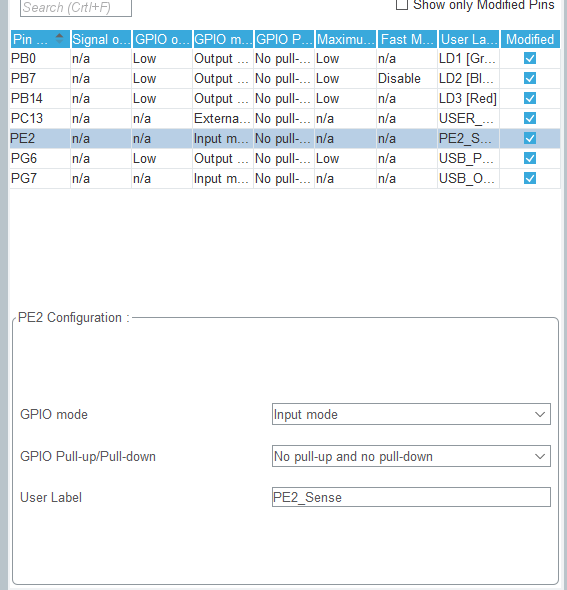
\includegraphics[width=6cm]{fig/Czujnik_przechylenia_KY020/polaczenie_modulu/GPIO.png}
%    \caption{Konfiguracja GPIO mikrokontrolera.}
%    \label{fig:my_label}
%\end{figure}
%\vspace{0.5cm}



\newpage

\section{Prezentacja działania układu}
Złożony został prosty układ w połączeniu z płytką NUCLEO-F767ZI, zgodny ze schematem z rys. \ref{fig:12}. Mikroprocesor został zaprogramowany tak, aby na stan wysoki z wyjścia czujnika odpowiadać zapaleniem się diody LD1. Działanie układu prezentuje się na zdjęciach poniżej. 

\begin{figure}[h]
\centering
\begin{subfigure}{.4\textwidth}
  \centering
  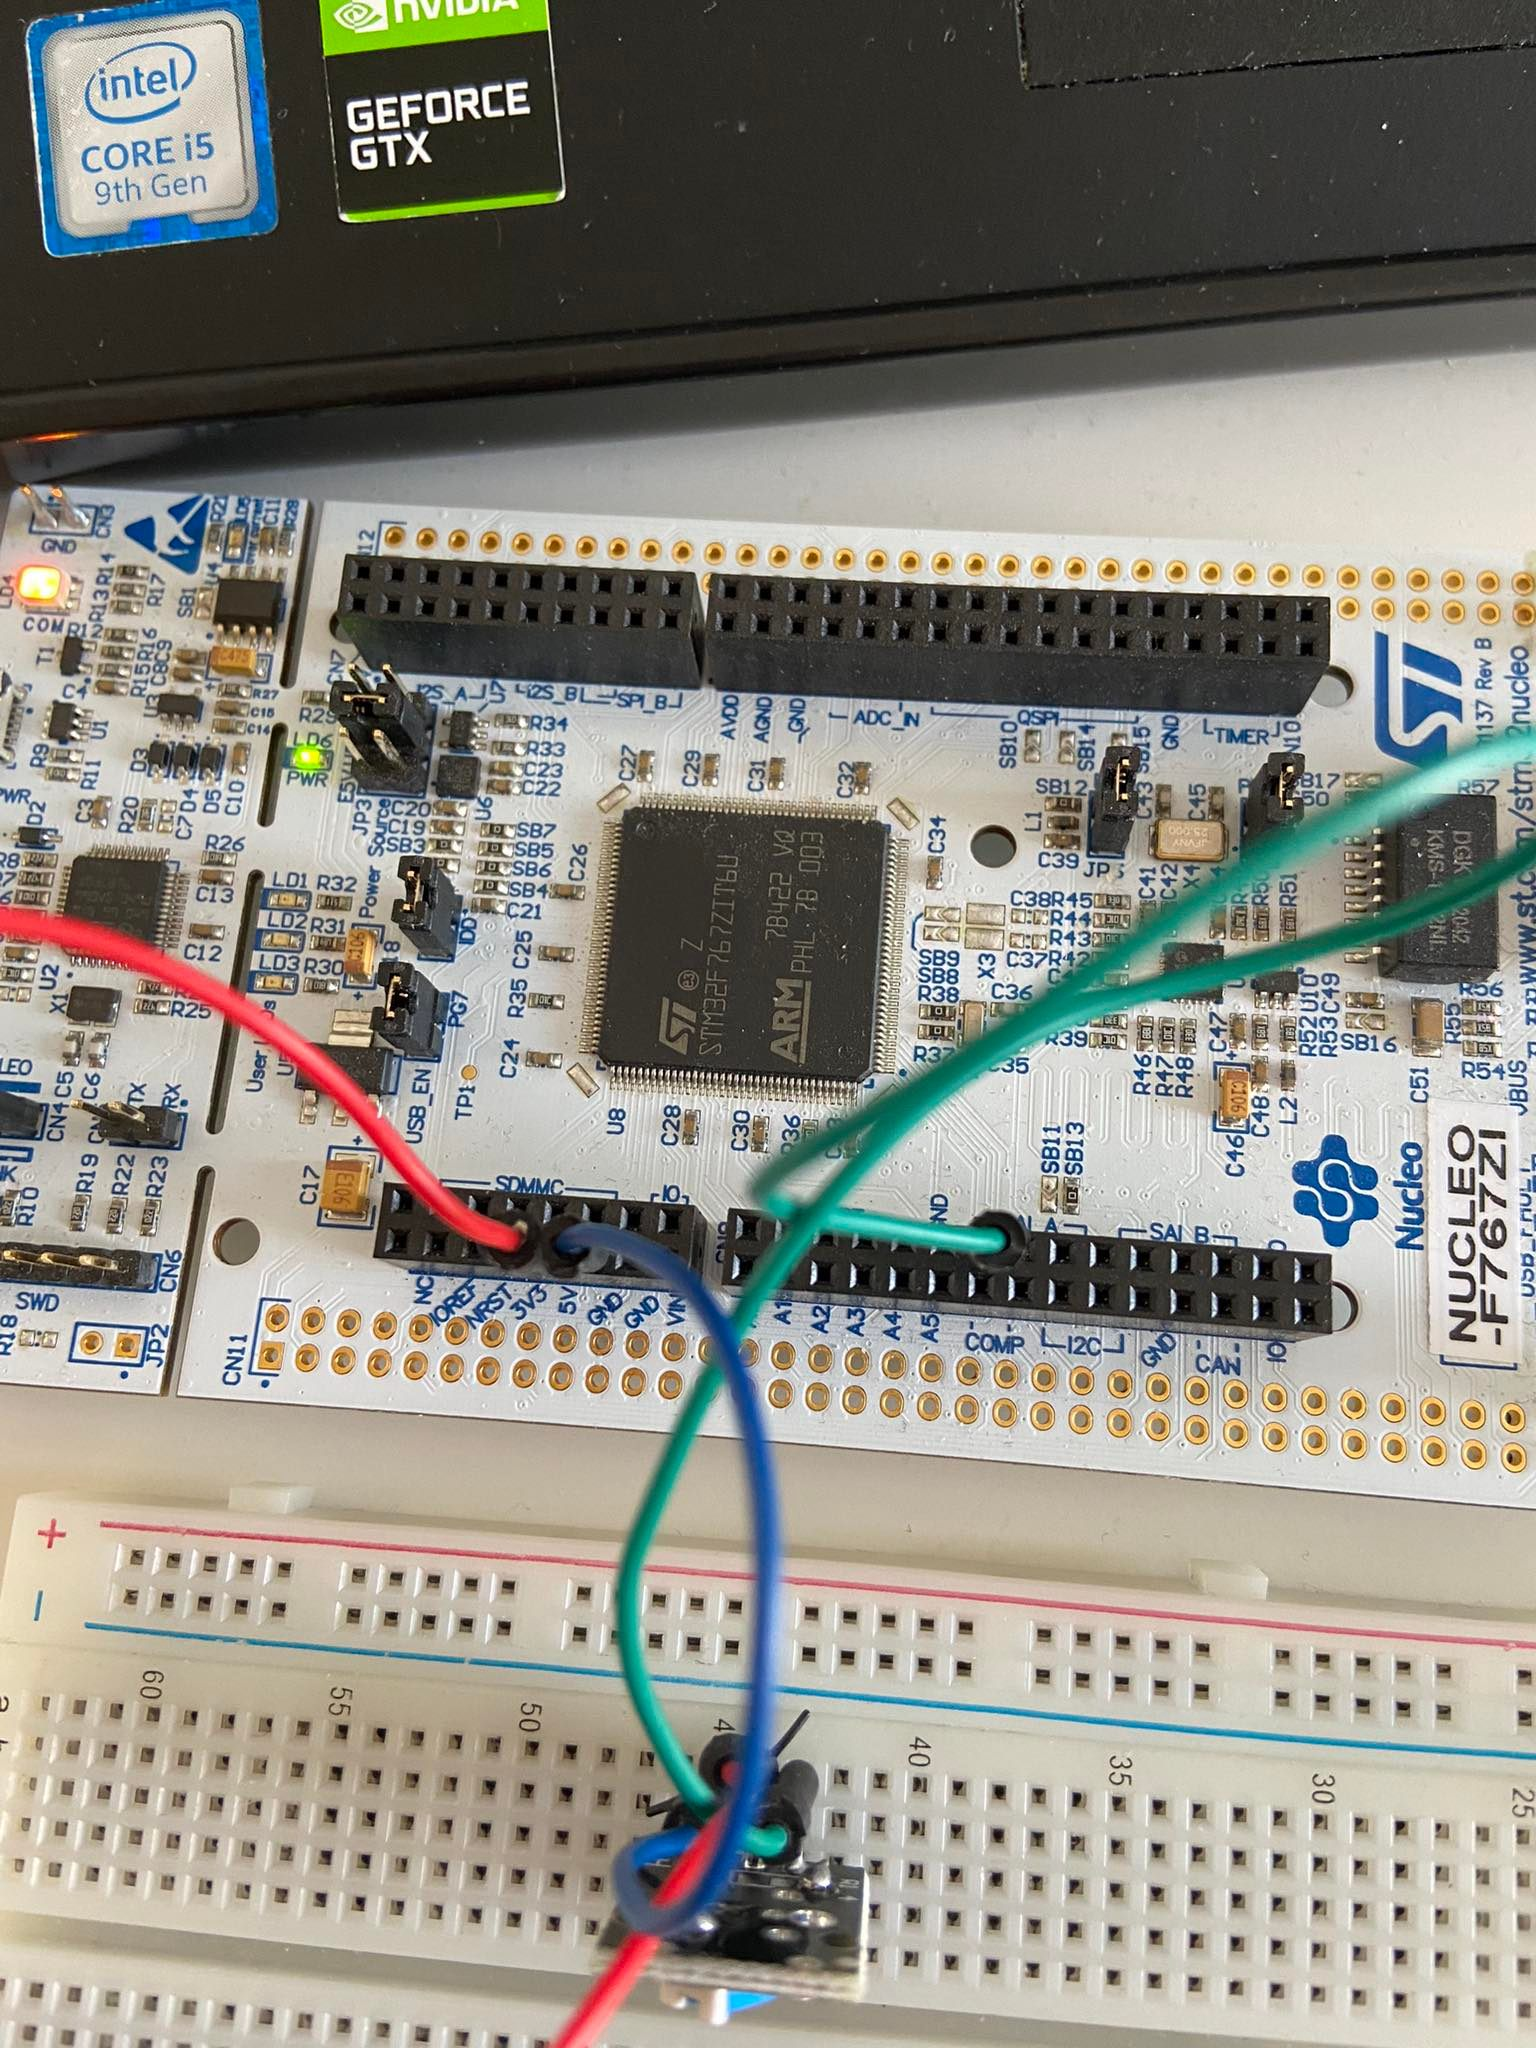
\includegraphics[width=.6\linewidth]{fig/Czujnik_przechylenia_KY020/działanie_ukladu/pulldown_dzialanie.jpg}
  \label{fig:12pd}
\end{subfigure}
\begin{subfigure}{.4\textwidth}
  \centering
  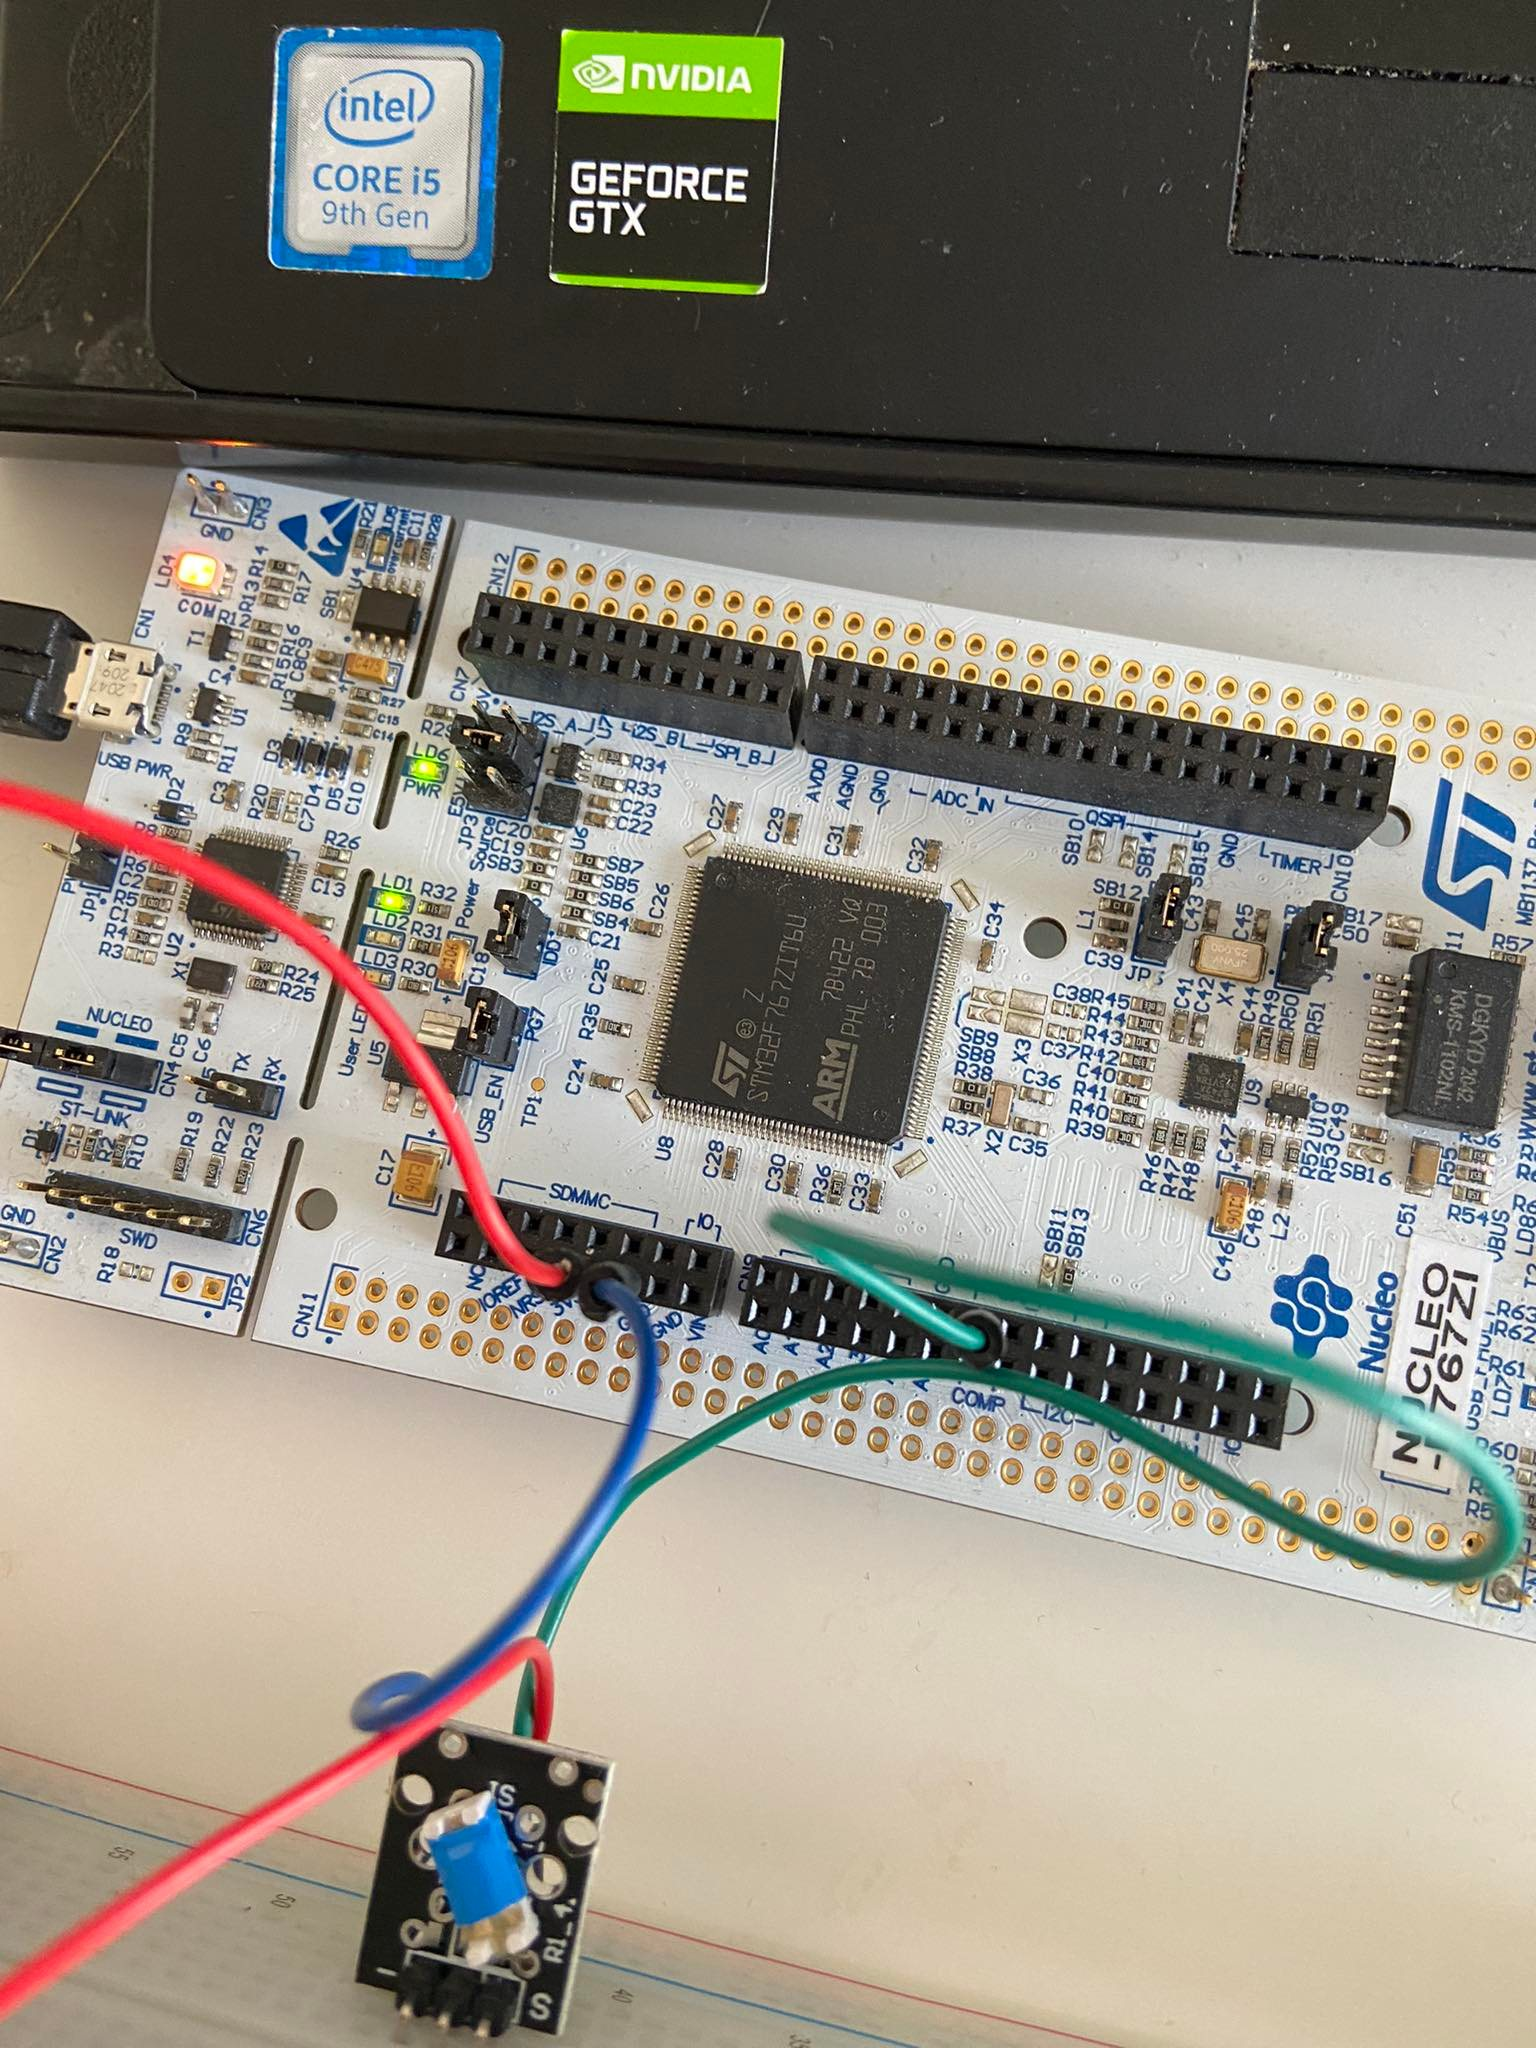
\includegraphics[width=.6\linewidth]{fig/Czujnik_przechylenia_KY020/działanie_ukladu/pulldown_dzialanie2.jpg}
  \label{fig:sub2}
\end{subfigure}
\caption{Konfiguracja rezystora ściągającego.}
\label{fig:12pu}
\end{figure}

\begin{figure}[h]
\centering
\begin{subfigure}{.4\textwidth}
  \centering
  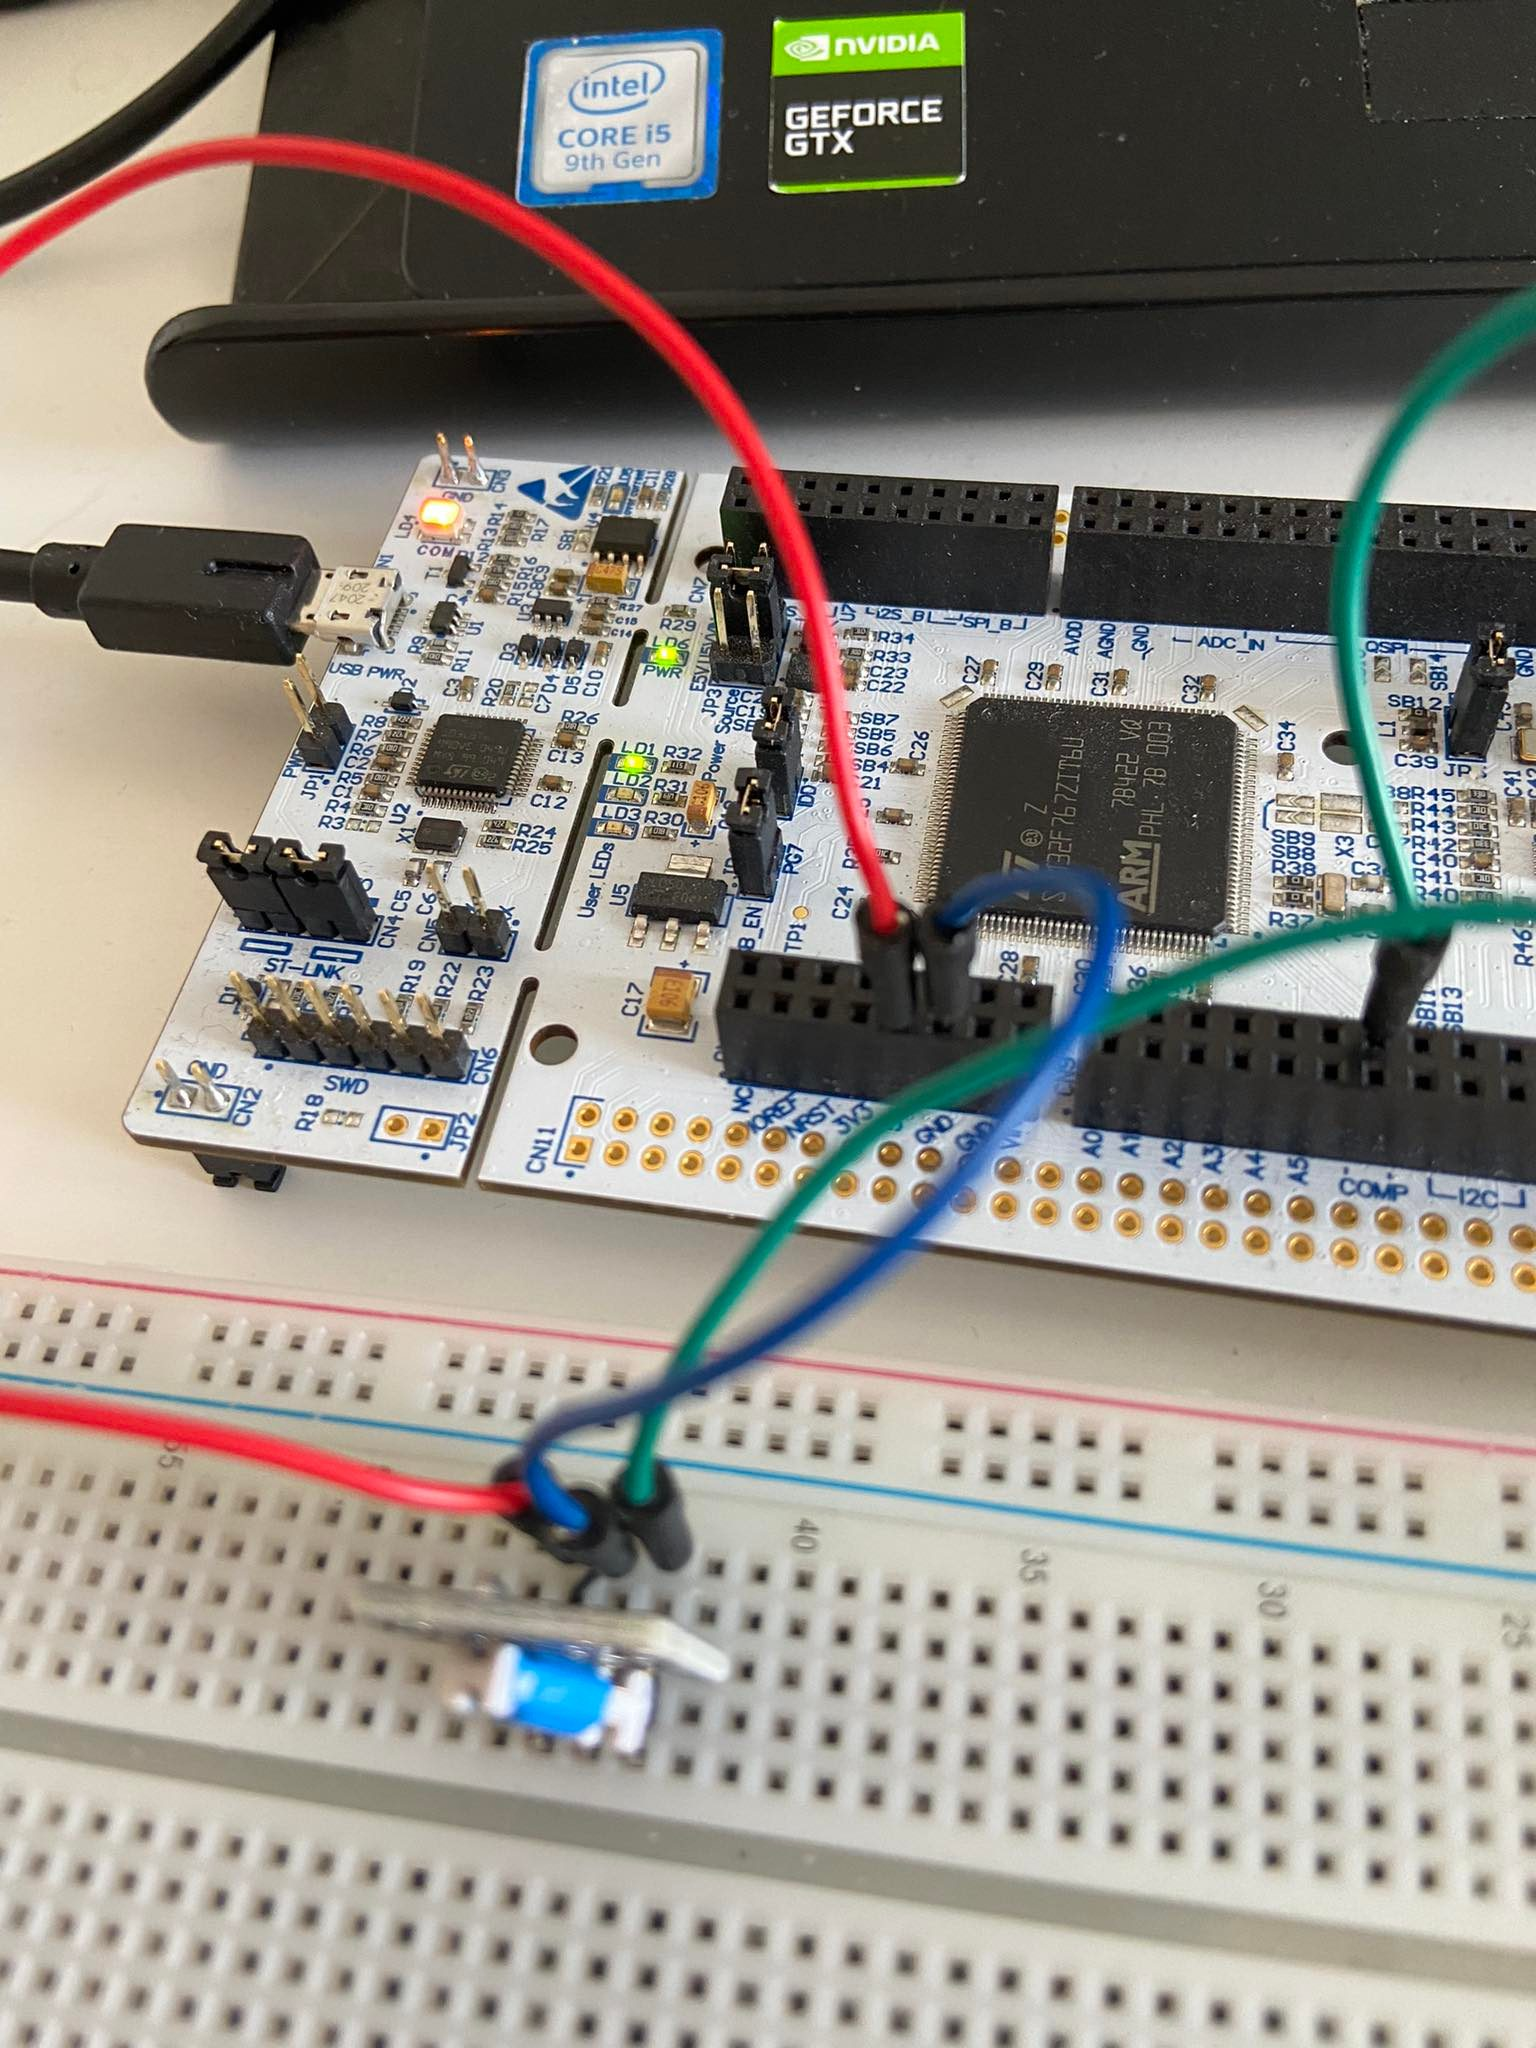
\includegraphics[width=.6\linewidth]{fig/Czujnik_przechylenia_KY020/działanie_ukladu/pullup_dzialanie.jpg}
  \label{fig:12pd}
\end{subfigure}
\begin{subfigure}{.4\textwidth}
  \centering
  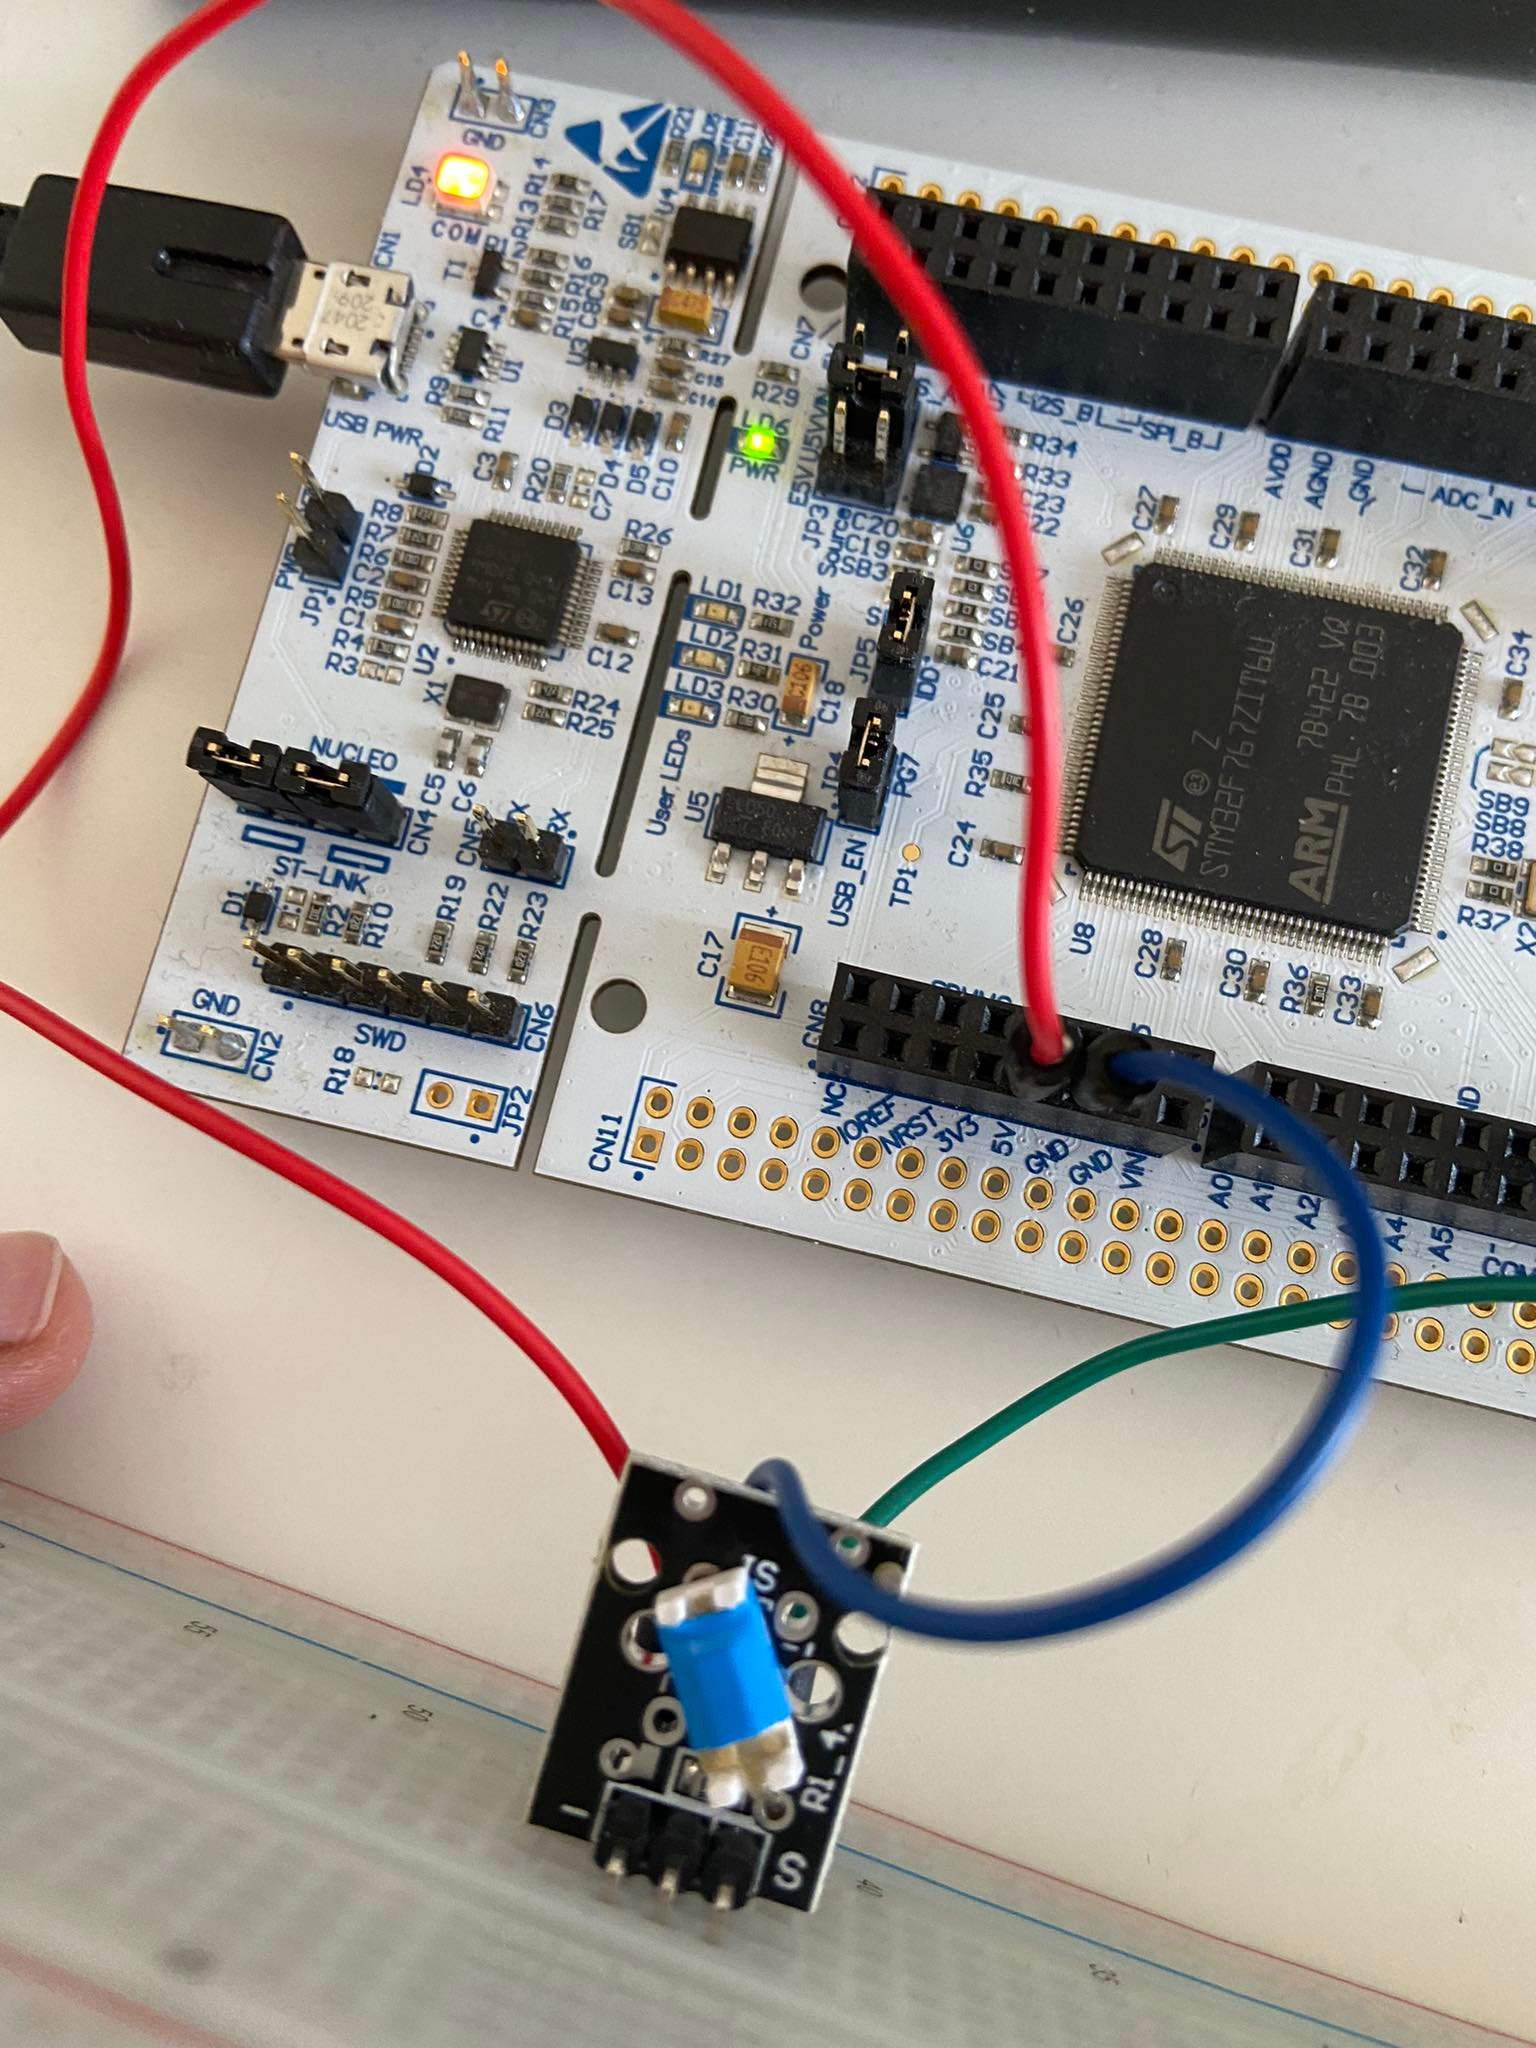
\includegraphics[width=.6\linewidth]{fig/Czujnik_przechylenia_KY020/działanie_ukladu/pullup_dzialanie2.jpg}
  \label{fig:sub2}
\end{subfigure}
\caption{Konfiguracja rezystora podciągającego.}
\label{fig:12pu}
\end{figure}

Jak widać na zamieszczonych zdjęciach, zmiana konfiguracji połączenia rezystora powoduje odwrócenie logiki działania czujnika, przez co dioda w trybie pull-down świeci się podczas wykrycia przechylenia, a w trybie pull-up kiedy ono nie występuje. 



\end{document}